% Set up the standalone document class
\documentclass{standalone}

% Input the preamble (<3)
% Preamble document

% Import tikz package
\usepackage{tikz}

% Import tikz libraries
\usetikzlibrary{shapes, arrows}
\usetikzlibrary{positioning, calc}

%----------- Create a fancy summing block
\tikzset{add/.style n args={4}{
		minimum width=6mm,
		path picture={
			\draw[black] 
			(path picture bounding box.south east) -- (path picture bounding box.north west)
			(path picture bounding box.south west) -- (path picture bounding box.north east);
			\node at ($(path picture bounding box.south)+(0,0.13)$)     {\tiny #1};
			\node at ($(path picture bounding box.west)+(0.13,0)$)      {\tiny #2};
			\node at ($(path picture bounding box.north)+(0,-0.13)$)    {\tiny #3};
			\node at ($(path picture bounding box.east)+(-0.13,0)$)     {\tiny #4};
		}
	}
}

%----------- Block style 1
\tikzstyle{block1} = [draw, fill=blue!20, rectangle, 
minimum height=3em, minimum width=6em, node distance=2.5cm]

%----------- Block style 2
\tikzstyle{block2} = [draw, fill=blue!20, rectangle, 
minimum height=3em, minimum width=3em, node distance=2.5cm]

%----------- Sum style
\tikzstyle{sum} = [draw, fill=blue!20, circle, node distance=2cm]

%----------- Input style
\tikzstyle{input} = [coordinate, node distance=4cm]

%----------- Output style
\tikzstyle{output} = [coordinate, node distance=4cm]

%----------- Pin style
\tikzstyle{pinstyle} = [pin edge={to-,thin,black}]

\begin{document}
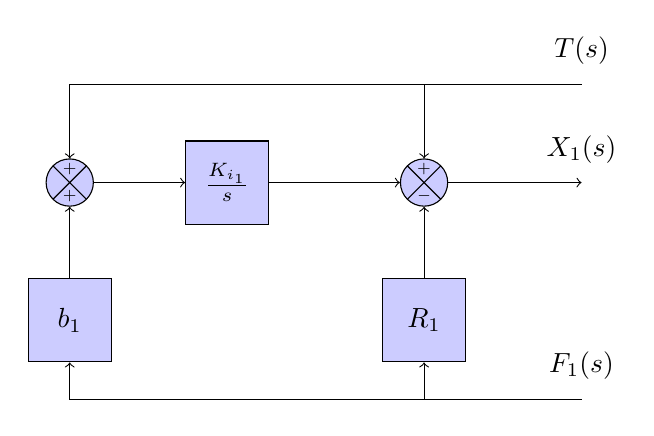
\begin{tikzpicture}	
	% Initial position node
	\node [coordinate] (c1) {};
	
	
	% Create nodes for upper leg
	\node [sum, above of=c1, add={$-$}{}{+}{}, node distance=3.5cm] (sum4) {};
	\node [coordinate, above of=sum4, node distance=1.25cm] (c10) {};
	\node [coordinate, right of=c10, node distance=2cm] (c12) {};
	\node [coordinate, right of=sum4, node distance=2cm] (c2) {};
	\node [coordinate, above of=c2] (c4) {};
	\node [block2, below of=sum4, node distance=1.75cm] (r1) {$R_1$};
	\node [coordinate, below of=r1] (c6) {};
	\node [coordinate, right of=c6, node distance=2cm] (c8) {};
	\node [block2, left of=sum4] (int1) {$\frac{K_{i_1}}{s}$};
	\node [sum, left of=int1, add={+}{ }{+}{ }] (sum6) {};
	\node [block2, below of=sum6, node distance=1.75cm] (b1) {$b_1$};
	
	
	% Connect nodes
	\draw [->] (sum4) -- node [at end, label=above:{$X_1(s)$}] {} (c2);
	\draw [->] (r1) -- (sum4);
	\draw [->] (b1) -- (sum6);
	\draw [->] (sum6) -- (int1);
	\draw [->] (int1) -- (sum4);
	\draw [->] (c8) -| node [at start, label=above:{$F_1(s)$}] {} (r1);
	\draw [->] (c8) -| (b1);
	\draw [->] (c12) -| node [at start, label=above:{$T(s)$}] {} (sum4);
	\draw [->] (c12) -| (sum6);
	
\end{tikzpicture}
\end{document}